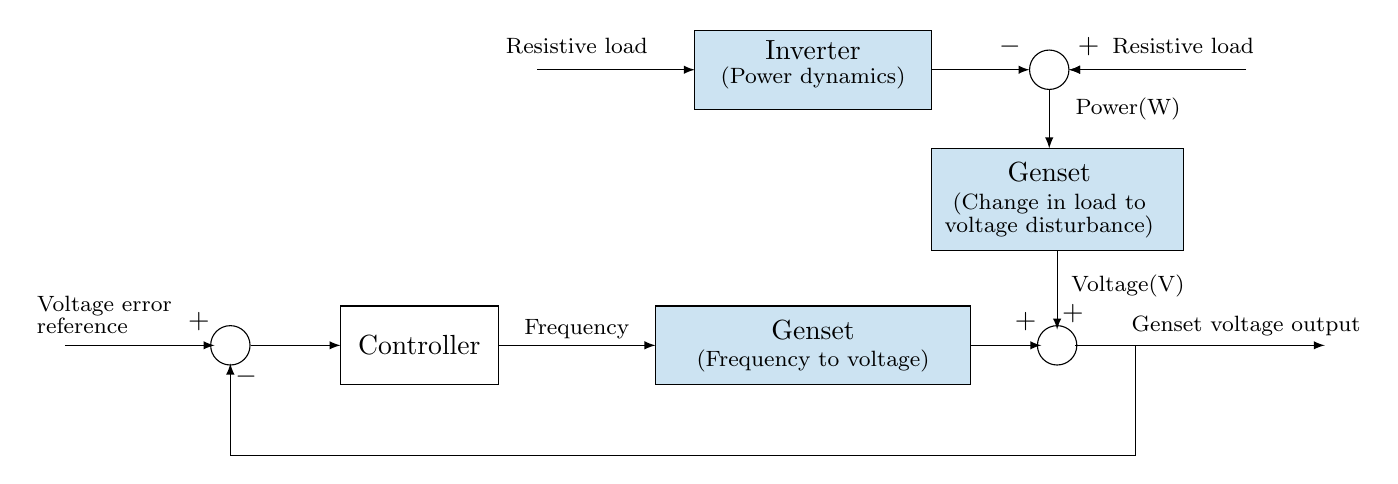
\begin{tikzpicture}
 \definecolor{mycolor1}{rgb}{0.00000,0.44700,0.74100} 
\draw  [fill=mycolor1!20](-5.5,2.5) rectangle (-1.5,1.5);
\draw [fill=mycolor1!20] (-2,4.5) rectangle (1.2,3.2);
\node at (-0.5,4.2) {\normalsize{Genset}};
\node at (-0.5,3.8) {\normalsize{\footnotesize{(Change in load to}}};
\node at (-0.5,3.5) {\normalsize{\footnotesize{voltage disturbance)}}};
\node at (-3.5,2.2) {\normalsize{Genset}};
\node at (-3.5,1.8) {\normalsize{\footnotesize{(Frequency to voltage)}}};

\draw [fill=mycolor1!20] (-5,6) rectangle (-2,5);
\draw [-latex] (-0.4,2) ellipse (0.25 and 0.25);
\draw [-latex](-1.5,2) -- (-0.6,2);
\draw [-latex](-0.4,3.2) -- (-0.4,2.2);
\draw [-latex] (-9.5,2.5) rectangle (-7.5,1.5);
\node at (-8.5,2) {Controller};
\draw [-latex](-7.5,2) -- (-5.5,2);

\node at (-0.2,2.4) {$+$};
\draw [-latex] (-10.9,2) ellipse (0.25 and 0.25);
\draw [-latex](-10.64,2) -- (-9.5,2);


\draw [-latex](-13,2) -- (-11.1,2);
\node at (-12.5,2.5) {\normalsize{\footnotesize{Voltage error}}};
\node at (-12.78,2.25) {\normalsize{\footnotesize{reference}}};
\draw [-latex](-0.17,2) -- (3,2);

\draw [-latex](0.6,2) -- (0.6,0.6) -- (-10.9,0.6) -- (-10.9,1.77);
\node at (-10.7,1.6) {$-$};
\node at (-11.3,2.3) {$+$};
\node at (-0.8,2.3) {$+$};
\node at (2,2.25) {\normalsize{\footnotesize{Genset voltage output}}};
\node at (-6.5,2.2) {\footnotesize{Frequency}};
\draw [-latex](2,5.5) -- (-0.25,5.5);
\node at (1.2,5.8) {\normalsize{\footnotesize{Resistive load}}};
\draw [-latex] (-0.5,5.5) ellipse (0.25 and 0.25);


\node at (-3.5,5.75) {\normalsize{Inverter}};
\node at (-3.5,5.4) {\normalsize{\footnotesize{(Power dynamics)}}};

\draw [-latex](2,5.5) -- (-0.25,5.5);
\draw [-latex](-2,5.5) -- (-0.75,5.5);
\draw [-latex](-0.5,5.25) -- (-0.5,4.5);
\draw [-latex](-7,5.5) -- (-5,5.5);

\node at (-6.5,5.8) {\normalsize{\footnotesize{Resistive load}}};
\node at (0.5,5) {\normalsize{\footnotesize{Power(W)}}};
\node at (0.5,2.75) {\normalsize{\footnotesize{Voltage(V)}}};

\node at (0,5.8) {$+$};
\node at (-1,5.8) {$-$};
\end{tikzpicture}